\section{Características}
\begin{frame}{Características}
\begin{itemize}
    \item Proporciona una alta ganancia de voltaje, pero atenúa la corriente ($A_i \leq 1$).
    \item Tiene baja impedancia de entrada, lo que es útil para ciertas aplicaciones.
    \item Utilizado en: circuitos de radiofrecuencia (RF), amplificadores de banda ancha.
\end{itemize}
\end{frame}

\section{Análisis y diseño}
\begin{frame}{Análisis y diseño}
Para el análisis y/o diseño de un circuito amplificador, se puede hacer uso de la propiedad de superposición.

\only<1>{
\begin{figure}[ht!]
    \centering
    \resizebox{0.5\textwidth}{!}{
        \begin{tikzpicture}
        	% Paths, nodes and wires:
        	\node[npn, rotate=90, yscale=-1](N1) at (-0, 2.75){} node[anchor=south] at (N1.text){$Q_1$};
        	\draw (3, 2.75) to[american resistor, l={$R_C$}] (3, 0);
        	\draw (-3, 0) to[american resistor, l={$R_1$}] (-0, 0);
        	\draw (-3, 0) to[american resistor, l={$R_E$}] (-3, 2.75);
        	\draw (-0, 0) to[american resistor, l={$R_2$}] (3, 0);
        	\draw (-0, 1.91) -- (-0, 0);
        	\draw (-3, 2.75) -- (-0.77, 2.75);
        	\draw (0.77, 2.75) -- (3, 2.75);
        	\draw (-3, 0) -- (-3, -1.75);
        	\draw (0.75, -1.75) to[battery, l={$V_{CC}$}] (-1, -1.75);
        	\draw (-3, -1.75) -- (-1, -1.75);
        	\draw (0.75, -1.75) -| (3, -0);
        \end{tikzpicture}
    }
    \caption{circuito equivalente para CC.}
\end{figure}
}
\only<2>{
\begin{figure}[ht!]
    \centering
    \resizebox{\textwidth}{!}{
        \begin{tikzpicture}
        	% Paths, nodes and wires:
        	\draw (3.25, 1.5) to[american resistor, l={$R_C$}] (3.25, -1.25);
        	\draw (-3.75, -1.25) to[american resistor, l={$R_E$}] (-3.75, 1.5);
        	\draw (5.25, 1.5) to[american resistor, l={$R_L$}] (5.25, -1.25);
        	\draw (-6.23, 1.5) to[sinusoidal voltage source, l={$v_i$}] (-6.25, -1.25);
        	\draw (-1.75, -1.25) to[american resistor, l={$h_{ib}$}] (-1.75, 1.5);
        	\draw (1.25, -1.25) to[american current source, l={$h_{fb} \cdot i_e$}] (1.25, 1.5);
        	\draw (-6.25, -1.25) -- (6.75, -1.25);
        	\node[ocirc] at (6.75, 1.5){};
        	\node[ocirc] at (6.75, -1.25){};
        	\draw (-6.23, 1.5) -| (-1.75, 1.5);
        	\draw (1.25, 1.5) -- (6.75, 1.5);
        \end{tikzpicture}
    }
    \caption{circuito equivalente para CA.}
\end{figure}
}
\end{frame}

\subsection{Polarización}
\begin{frame}{Polarización}
El transistor tiene tres regiones de trabajo: activa, corte y saturación. 
La polarización consiste en definir los componentes de red adecuados, que permitan
que el transistor opere en una región y en un punto determinados. Condición necesaria para
operación en región activa es una polarización emisor-base directa y una polarización
colector-base inversa.
\end{frame}

\subsubsection{Máxima Excursión Simétrica}
\begin{frame}{Máxima Excursión Simétrica}
En particular, se busca ubicar el punto de operación Q en la recta de carga de tal forma que la señal de salida pueda desplazarse con la mayor amplitud
posible antes de alcanzar las regiones de saturación o corte.

Este criterio se conoce como polarización para máxima excursión simétrica (MES).

\begin{figure}[!ht]
  \centering
  \resizebox{0.5\textwidth}{!}{
      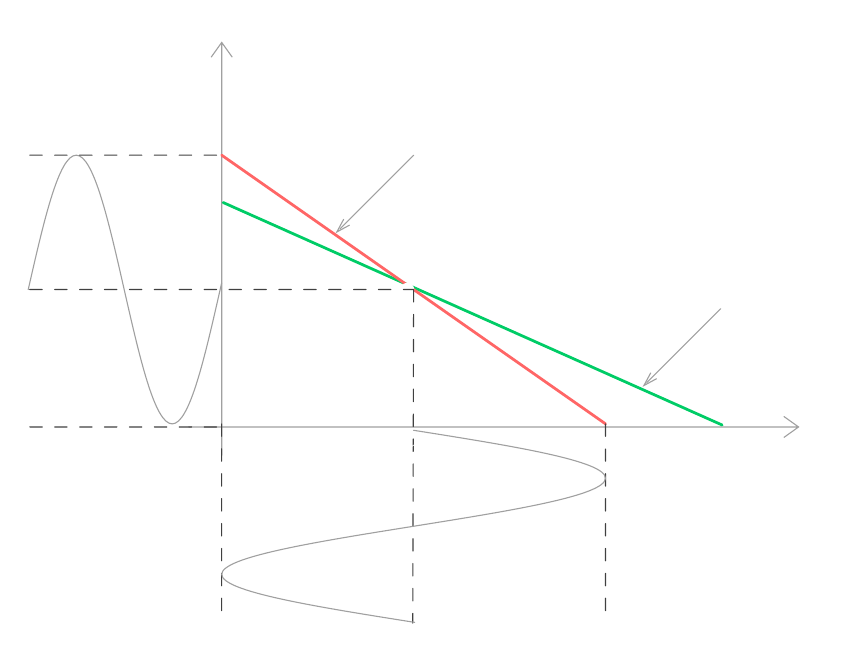
\begin{tikzpicture}[x=0.75pt,y=0.75pt,yscale=-1,xscale=1,
                          line cap=round, text=white]
        \definecolor{axis}{HTML}{A0A0A0}
        \definecolor{grid}{HTML}{404040}
        \definecolor{acc1}{HTML}{00CC66}
        \definecolor{acc2}{HTML}{FF6666}
    
        % Ejes
        \draw[axis] (178.6,264.42) -- (472.39,264.42)
                    (194.46,79.16) -- (194.46,278.05)
                    (465.39,259.42) -- (472.39,264.42) -- (465.39,269.42)
                    (189.46,86.16)  -- (194.46,79.16) -- (199.46,86.16);
    
        % Recta verde (acento)
        \draw[acc1, line width=1] (195.14,156.28) -- (435.55,263.48);
    
        % Recta roja
        \draw[acc2, line width=1] (194.45,133.48) -- (379.39,262.94);
    
        % Punto Q negro -> blanco
        \draw[fill=white, draw=white] (283.94,198.21)
          circle [x radius=2.98, y radius=2.98];
    
        % Curva izquierda
        \draw[axis] (101.24,198.21) .. controls (108.78,165.05) and (115.99,133.48) ..
          (124.35,133.48) .. controls (132.72,133.48) and (139.93,165.05) ..
          (147.47,198.21) .. controls (155.01,231.37) and (162.22,262.94) ..
          (170.59,262.94) .. controls (178.96,262.94) and (186.17,231.37) ..
          (193.71,198.21) .. controls (193.95,197.13) and (194.2,196.04) ..
          (194.45,194.96);
    
        % Guías punteadas
        \draw[grid, dash pattern={on 4.5pt off 4.5pt}]
          (101.98,133.48) -- (194.45,133.48)
          (101.99,264.42) -- (194.46,264.42)
          (101.98,198.21) -- (286.92,198.21)
          (286.92,198.21) -- (286.51,358.87)
          (379.39,262.94) -- (379.39,355.41)
          (194.45,262.94) -- (194.45,355.41);
    
        % Onda derecha
        \draw[axis] (286.88,266.02) .. controls (334.25,273.53) and (379.35,280.72) ..
          (379.35,289.09) .. controls (379.36,297.46) and (334.27,304.69) ..
          (286.91,312.26) .. controls (239.54,319.82) and (194.45,327.06) ..
          (194.46,335.42) .. controls (194.46,343.79) and (239.56,350.98) ..
          (286.93,358.49) .. controls (287.09,358.52) and (287.25,358.54) ..
          (287.42,358.57);
    
        % Flechas
        \draw[axis] (286.92,133.48) -- (251.34,169.06);
        \draw[axis, shift={(249.93,170.47)}, rotate=315] (6.56,-1.97) --
          (0,0) -- (6.56,1.97);
        \draw[axis] (434.87,207.46) -- (399.3,243.03);
        \draw[axis, shift={(397.88,244.45)}, rotate=315] (6.56,-1.97) --
          (0,0) -- (6.56,1.97);
    
        % Textos
        \draw (292.24,275.1) node[font=\tiny] {$\displaystyle V_{CEQ}$};
        \draw (172.55,182.55) node[font=\tiny] {$\displaystyle I_{CQ}$};
        \draw (202.71,79.9)   node[font=\tiny] {$\displaystyle I_{C}$};
        \draw (473.73,254.25) node[font=\tiny] {$\displaystyle V_{CB}$};
        \draw (287.64,119.68) node[font=\scriptsize] {$\displaystyle m_{ca}$};
        \draw (432.14,192.26) node[font=\scriptsize] {$\displaystyle m_{cc}$};
        \draw (383.71,272.76) node[font=\tiny] {$\displaystyle 2V_{CEQ}$};
        \draw (166.67,117.46) node[font=\tiny] {$\displaystyle 2I_{CQ}$};
        \draw (285.64,180.08) node[font=\scriptsize] {$\displaystyle Q_{MES}$};
      \end{tikzpicture}
    }
  \caption{gráfica punto $Q_{MES}$.}
  \label{fig:gráfica-mes}
\end{figure}
\end{frame}

\begin{frame}[allowframebreaks]{Malla de salida}
\begin{figure}[H]
    \centering
    \begin{minipage}{0.4\textwidth}
        \centering
        \resizebox{0.6\textwidth}{!}{
        \begin{tikzpicture}
            \node[npn](N1) at (1.59, 2){} node[anchor=west] at (N1.text){$Q1$};
            \draw (1.59, 1.25) to[american resistor, l={$R_E$}] (1.59, -1);
            \draw (1.59, 5.02) to[american resistor, l={$R_c$}] (1.59, 2.77);
            \draw (1.59, -1) -| (1.59, -1.25);
            \node[vcc](N2) at (1.59, 6){} node[anchor=south] at (N2.text){$V_{cc}$};
            \draw (1.59, 5.25) -| (1.59, 6);
            \node[ground] at (1.59, -1.75){};
            \draw (1.59, -1.25) -| (1.59, -1.75);
            \draw (-1.66, 2) to[american resistor, l={$R_B$}] (-1.66, -0.25);
            \draw (-1.66, -0.25) to[battery1, l={$V_{BB}$}] (-1.66, -1.5);
            \draw (-1.66, 2) -| (0.75, 2);
            \draw (-1.66, -1.5) -| (-1.66, -1.75) -- (1.59, -1.75);
            \draw (1.59, 5.02) -| (1.59, 5.25);
        \end{tikzpicture}
    }
        \caption{Circuito para CC simplificado por Thévenin.}
        \label{fig:malla-salida}
    \end{minipage}%
    \begin{minipage}{0.45\textwidth}
        \centering
        Donde $R_{B}$ es la resistencia equivalente y $V_{BB}$ es la tensión de Thévenin:
        \begin{align}
            R_{B} &= R_1||R_2=\frac{R_1 R_2}{R_1 + R_2} \label{ec:thevenin-rb}\\[6pt]
            V_{BB} &= V_{CC} \cdot \frac{R_1}{R_1 + R_2} \label{ec:thevenin-vbb}
        \end{align}
        Se debe determinar los valores de $R_B$ y $V_{BB}$ con el objetivo de polarizar
        el transistor para MES.
    \end{minipage}
\end{figure}

Aplicando LKV a la malla de salida:

\begin{align}
    V_{CC} - I_{CQ}R_C - V_{CBQ} + \frac{I_{CQ}}{\beta}R_B - V_{BB} &= 0 \label{ec:malla-salida-cc}
\end{align}

\begin{figure}[!ht]
  \centering
  \begin{minipage}{0.45\textwidth}
  \resizebox{0.6\textwidth}{!}{
    \begin{tikzpicture}
    	% Paths, nodes and wires:
    	\node[npn, rotate=90, yscale=-1] at (-0, 1.5){};
    	\draw (2, 1.5) to[american resistor, l={$R_C$}] (2, -1.25);
    	\draw (4, 1.5) to[american resistor, l={$R_L$}] (4, -1.25);
    	\draw (-0, 0.66) -- (-0, -1.25) -- (4, -1.25);
    	\draw (0.75, 1.5) -- (4, 1.5);
    	\node[ground] at (-0, -1.25){};
    \end{tikzpicture}
    }
    \caption{malla de salida para $CA$.}
    \label{fig:malla-salida-ca}
  \end{minipage}
  \begin{minipage}{0.45\textwidth}
    \centering
    LKV:
    \begin{align}
        \hat{v}_{cb} &= \hat{\imath}_c(R_C ||R_L) \nonumber \\[6pt]
        \hat{v}_{cb} &= \hat{\imath}_c\frac{R_C R_L}{R_C + R_L} \nonumber \\[6pt]
        \hat{v}_{cb} &= \hat{\imath}_c(R_{CA}) \label{ec:malla-salida-ca}
    \end{align}
  \end{minipage}
\end{figure}

Por definición de MES, se tiene que la amplitud pico de la señal de salida es:
\begin{align*}
    \hat{v}_{cb} &= V_{CBQ}\\[6pt]
    \hat{\imath}_c &= I_{CQ}
\end{align*}

Reemplazando esto en la ecuación \ref{ec:malla-salida-ca}:

\begin{align*}
    V_{CBQ} &= I_{CQ}(R_{CA})
\end{align*}

Y reemplazando esta última igualdad en la ecuación \ref{ec:malla-salida-cc}:

\begin{align}
    V_{CC} - I_{CQ}R_C - V_{CBQ} + \frac{I_{CQ}}{\beta}R_B - V_{BB} &= 0 \nonumber \\[6pt]
    V_{CC} - I_{CQ}R_C - I_{CQ}(R_{CA}) + \frac{I_{CQ}}{\beta}R_B - V_{BB} &= 0 \nonumber \\[6pt]
    I_{CQ} = \frac{V_{CC} - V_{BB}}{R_C-\frac{R_B}{\beta} + (R_{CA})} \\[6pt]
    I_{CQ_{MES}} = \frac{V_{CC} - V_{BB}}{(R_{CC}) + (R_{CA})} \label{ec:iq-mes}
\end{align}

\begin{minipage}[][\textheight][]{\textwidth}
Despejando para $V_{CB}$:
\begin{align}
    V_{CC} - I_{CQ}R_C - V_{CBQ} + \frac{I_{CQ}}{\beta}R_B - V_{BB} &= 0 \nonumber \\[6pt]
    V_{CBQ_{MES}} = V_{CC} - V_{BB} - I_{CQ_{MES}}(R_{CC}) \label{ec:vcb-mes}
\end{align}
\end{minipage}

\end{frame}

\begin{frame}[allowframebreaks]{Determinación de $V_{BB}$ y $R_B$}
Para determinar $V_{BB}$ se tiene que aplicar LKV a la malla de entrada.

\begin{figure}[H]
    \centering
    \begin{minipage}{0.4\textwidth}
        \centering
        \resizebox{0.6\textwidth}{!}{
            \begin{tikzpicture}
              % Paths, nodes and wires:
              \node[npn](N1) at (0, 0){} node[anchor=west] at (N1.text){$Q1$};
              \draw (0, -0.77) to[american resistor, l={$R_E$}] (0, -3);
              \draw (0, 3.02) to[american resistor, l={$RC$}] (0, 0.77);
              \draw (0, -3) -| (0, -3.25);
              \node[vcc](N2) at (0, 3.02){} node[anchor=south] at (N2.text){$V{cc}$};
              \node[ground] at (0, -3.75){};
              \draw (0, -3.25) -| (0, -3.75);
              \draw (-3.25, 0) to[american resistor, l={$RB$}] (-3.25, -2.25);
              \draw (-3.25, 0) -- (-0.84, 0);
              \draw (-3.25, -3.5) -| (-3.25, -3.75) -- (0, -3.75);
              \draw (-3.25, -2.25) to[battery, l={$V{BB}$}] (-3.25, -3.5);
            \end{tikzpicture}
    }
        \caption{Circuito para CC simplificado por Thévenin.}
        \label{fig:malla-entrada}
    \end{minipage}%
    \begin{minipage}{0.4\textwidth}
        \centering
        LKV:
        \begin{gather}
            V_{BB} - I_{BQ}R_B - V_{BE}-I_{EQ}R_E = 0 \nonumber\\[6pt]
            V_{BB} - \frac{I_{CQ}}{\beta}R_B - V_{BE}-I_{CQ}R_E = 0 \nonumber\\[6pt]
            I_{CQ} = \frac{V_{BB} - V_{BE}}{\frac{R_B}{\beta}+R_E}
        \end{gather}
    \end{minipage}
\end{figure}

Igualando esta ecuación con la ecuación de $I_{CQ_{MES}}$ (Ec. \ref{ec:iq-mes}):

\begin{gather}
    \frac{V_{CC}-V_{BB}}{R_{CC} + R_{CA}}= \frac{V_{BB}-V_{BE}}{\frac{R_B}{\beta}+R_E} \nonumber\\[6pt]
    V_{CC}(\frac{R_B}{\beta}+R_E) - V_{BB}(\frac{R_B}{\beta}+R_E) = V_{BB}(R_{CC}+R_{CA}) - V_{BE}(R_{CC}+R_{CA}) \nonumber\\[6pt]
    V_{BB} = \frac{V_{CC}(\frac{R_B}{\beta}+R_E) + V_{BE}(R_{CC}+R_{CA})}{\frac{R_B}{\beta}+R_E + R_{CC} + R_{CA}} \nonumber\\[6pt]
    V_{BB} = \frac{V_{CC}(\frac{R_B}{\beta}+R_E) + V_{BE}(R_C-\frac{R_B}{\beta}+R_C||R_L)}{R_E + R_C + R_C||R_L} \label{ec:vbb}\\[6pt]
    \nonumber
\end{gather}

$R_B$ se puede determinar considerando el siguiente criterio de diseño:

\begin{equation}
    R_E  \gg \frac{R_b}{\beta} \therefore R_E = 10\frac{R_B}{\beta} \therefore \frac{R_B}{\beta} = \frac{R_E}{10} \label{ec:criterio-diseño}
\end{equation}

Finalmente, para determinar el valor de $R_1$ y $R_2$, se consideran las ecuaciones (\ref{ec:thevenin-rb}) y (\ref{ec:thevenin-vbb}), resultantes de aplicar Thévenin a la malla de entrada del circuito 
amplificador, y la ecuación \ref{ec:criterio-diseño},
resultante de establecer el criterio de diseño:

\begin{align*}
    R_B &= R_1||R_2=\frac{R_1 R_2}{R_1 + R_2} \tag{\ref{ec:thevenin-rb}}\\[6pt]
    V_{BB} &= V_{CC} \cdot \frac{R_1}{R_1 + R_2} \tag{\ref{ec:thevenin-vbb}}\\[6pt]
    R_B &= \boxed{\beta \frac{R_E}{10}} \tag{\ref{ec:criterio-diseño}}
\end{align*}

Ahora que los valores de $R_B$ y $V_{BB}$ se pueden determinar, se puede proceder a 
despejar $R_1$ y  $R_2$ de las ecuaciones correspondientes, obteniendo:

\begin{figure}[!ht]
    \centering
    \begin{minipage}[][\textheight][]{0.45\textwidth}
    \begin{equation}
        \boxed{R_1 = \frac{R_B}{1-\frac{V_{BB}}{V_{CC}}}}
        \label{eq:r1}
    \end{equation}
    \end{minipage}
    \begin{minipage}[][\textheight][]{0.45\textwidth}
    \begin{equation}
        \boxed{R_2 = \frac{V_{CC}R_B}{V_{BB}}}
        \label{eq:r2}
    \end{equation}
    \end{minipage}
\end{figure}
\end{frame}

\subsection{Rectas de carga}
\begin{frame}[fragile,allowframebreaks]{Rectas de carga}
    Recordando la Ec. (\ref{ec:malla-salida-cc}) de la malla de salida del circuito para CC
    y despejando para $V_{CBQ_{MES}}$

\begin{gather}
    V_{CC} - I_{CQ}R_C - V_{CBQ} + \frac{I_{CQ}}{\beta}R_B - V_{BB} = 0 \nonumber \\[6pt]
    V_{CBQ} = V_{CC} - V_{BB} - (R_C - \frac{R_B}{\beta})I_{CQ} \label{ec:recta-carga-cc}
\end{gather}

La Ec. (\ref{ec:recta-carga-cc}) corresponde a la recta de carga para CC.

Recordando la Ec. (\ref{ec:malla-salida-ca}) de la malla de salida del circuito para CA y
considerando que la recta tiene una ordenada al origen que hay que determinar:

\begin{gather}
v_{cb} = V_{CC}'-i_c\frac{R_C R_L}{R_C + R_L} \nonumber
\end{gather}

Se puede determinar el valor de $V_{CC}$ evaluando la ecuación para un punto conocido y
despejando. Considerando el punto $Q_{MES}$:

\begin{align*}
V_{CBQ_{MES}} = V_{CC}'-I_{CQ_{MES}}\frac{R_C R_L}{R_C + R_L} \\[6pt]
V_{CC}' = V_{CBQ_{MES}} + I_{CQ_{MES}}\frac{R_C R_L}{R_C + R_L}
\end{align*}

Por lo tanto:

\begin{align}
    v_{cb} &= (V_{CBQ_{MES}} + I_{CQ_{MES}}\frac{R_C R_L}{R_C + R_L})-i_c\frac{R_C R_L}{R_C + R_L} \label{ec:recta-carga-ca}
\end{align}

Esta Ec. (\ref{ec:recta-carga-ca}) corresponde a la recta de carga para CA.

\begin{figure}
    \centering
    \resizebox{0.8\textwidth}{!}{      
    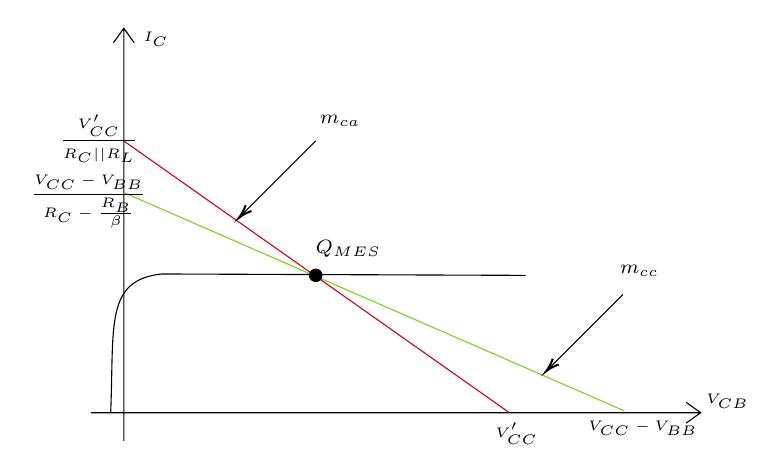
\begin{tikzpicture}[x=0.75pt,y=0.75pt,yscale=-1,xscale=1]
        %uncomment if require: \path (0,538); %set diagram left start at 0, and has height of 538
        %Shape: Axis 2D [id:dp5849296416796758] 
        \draw  (184.93,249.75) -- (478.72,249.75)(200.79,64.5) -- (200.79,263.39) (471.72,244.75) -- (478.72,249.75) -- (471.72,254.75) (195.79,71.5) -- (200.79,64.5) -- (205.79,71.5)  ;
        %Straight Lines [id:da0025452687883318337] 
        \draw [color={rgb, 255:red, 126; green, 211; blue, 33 }  ,draw opacity=1 ][fill={rgb, 255:red, 126; green, 211; blue, 33 }  ,fill opacity=1 ]   (200.83,143.7) -- (441.88,248.82) ;
        %Straight Lines [id:da4207709647475807] 
        \draw [color={rgb, 255:red, 208; green, 2; blue, 27 }  ,draw opacity=1 ]   (200.78,118.82) -- (386.5,249.7) ;
        %Shape: Ellipse [id:dp6638447632450213] 
        \draw  [fill={rgb, 255:red, 0; green, 0; blue, 0 }  ,fill opacity=1 ] (290.27,183.55) .. controls (290.27,181.9) and (291.61,180.56) .. (293.25,180.56) .. controls (294.9,180.56) and (296.23,181.9) .. (296.23,183.55) .. controls (296.23,185.19) and (294.9,186.53) .. (293.25,186.53) .. controls (291.61,186.53) and (290.27,185.19) .. (290.27,183.55) -- cycle ;
        %Straight Lines [id:da5509689272628648] 
        \draw    (293.25,118.82) -- (257.68,154.39) ;
        \draw [shift={(256.26,155.8)}, rotate = 315] [color={rgb, 255:red, 0; green, 0; blue, 0 }  ][line width=0.75]    (6.56,-1.97) .. controls (4.17,-0.84) and (1.99,-0.18) .. (0,0) .. controls (1.99,0.18) and (4.17,0.84) .. (6.56,1.97)   ;
        %Straight Lines [id:da7225229987184748] 
        \draw    (441.21,192.79) -- (405.63,228.37) ;
        \draw [shift={(404.22,229.78)}, rotate = 315] [color={rgb, 255:red, 0; green, 0; blue, 0 }  ][line width=0.75]    (6.56,-1.97) .. controls (4.17,-0.84) and (1.99,-0.18) .. (0,0) .. controls (1.99,0.18) and (4.17,0.84) .. (6.56,1.97)   ;
        %Curve Lines [id:da8301807553903576] 
        \draw    (194.46,249.42) .. controls (196.17,207.37) and (191.7,185.9) .. (219.03,182.9) ;
        %Straight Lines [id:da4061818256505698] 
        \draw    (219.03,182.9) -- (394.37,183.57) ;
        
        % Text Node
        \draw (209.05,65.23) node [anchor=north west][inner sep=0.75pt]  [font=\tiny] [align=left] {$\displaystyle I_{C}$};
        % Text Node
        \draw (480.06,239.58) node [anchor=north west][inner sep=0.75pt]  [font=\tiny] [align=left] {$\displaystyle V_{CB}$};
        % Text Node
        \draw (293.97,105.02) node [anchor=north west][inner sep=0.75pt]  [font=\scriptsize] [align=left] {$\displaystyle m_{ca}$};
        % Text Node
        \draw (438.48,177.6) node [anchor=north west][inner sep=0.75pt]  [font=\scriptsize] [align=left] {$\displaystyle m_{cc}$};
        % Text Node
        \draw (291.97,165.42) node [anchor=north west][inner sep=0.75pt]  [font=\scriptsize] [align=left] {$\displaystyle Q_{MES}$};
        % Text Node
        \draw (423.27,252.54) node [anchor=north west][inner sep=0.75pt]  [font=\tiny] [align=left] {$\displaystyle V_{CC} -V_{BB}$};
        % Text Node
        \draw (154.73,134.14) node [anchor=north west][inner sep=0.75pt]  [font=\tiny] [align=left] {$\displaystyle \frac{V_{CC} -V_{BB}}{R_{C} -\frac{R_{B}}{\beta }}$};
        % Text Node
        \draw (378.53,253.4) node [anchor=north west][inner sep=0.75pt]  [font=\tiny] [align=left] {$\displaystyle V'_{CC}$};
        % Text Node
        \draw (168.53,105.07) node [anchor=north west][inner sep=0.75pt]  [font=\tiny] [align=left] {$\displaystyle \frac{V'_{CC}}{R_{C} ||R_{L}}$};
    \end{tikzpicture}
    }
    \caption{rectas de carga.}
    \label{fig:rectas-de-carga}
\end{figure}

\end{frame}

\subsection{Pequeña señal}
\begin{frame}[allowframebreaks]{Análisis para pequeñal señal}
Para el análisis de pequeña señal, se considera un circuito equivalente del transistor en
base común.

\begin{figure}
    \centering
    \resizebox{0.6\textwidth}{!}{
    \begin{tikzpicture}
    	% Paths, nodes and wires:
    	\draw (3.375, 1.25) to[american resistor, l={$\frac{1}{h_{ob}}$}] (3.375, -1.5);
    	\draw (-4.625, 1.25) to[american resistor, l={$h_{ib}$}] (-2.875, 1.25);
    	\draw (1.5, 1.25) to[american current source, mirror, l_={$h_{fb} \cdot i_e$}] (1.5, -1.5);
    	\draw (-1.5, 1.25) to[american voltage source, l_={$h_{rb} \cdot v_{eb}$}] (-1.5, -1.5);
    	\draw (-2.875, 1.25) -- (-1.5, 1.25);
    	\draw (1.5, 1.25) -- (5.25, 1.25);
    	\draw (-4.625, 1.25) -- (-5.25, 1.25);
    	\draw (5.125, -1.5) -| (-5.25, -1.5);
    	\node[shape=rectangle, draw, line width=1pt, minimum width=9.215cm, minimum height=4.465cm] at (0, 0){};
    	\node[ground] at (-0, -1.5){};
    	\node[shape=rectangle, minimum width=0.715cm, minimum height=0.715cm] at (0, -1.25){} node[anchor=north west, align=left, text width=0.327cm, inner sep=6pt] at (-0.375, -0.875){B};
    	\node[shape=rectangle, minimum width=0.652cm, minimum height=0.59cm] at (5.594, 1.25){} node[anchor=north west, align=left, text width=0.264cm, inner sep=6pt] at (5.25, 1.562){C};
    	\node[shape=rectangle, minimum width=0.59cm, minimum height=0.59cm] at (-5.562, 1.25){} node[anchor=north west, align=left, text width=0.202cm, inner sep=6pt] at (-5.875, 1.562){E};
    	\node[ocirc] at (5.25, 1.25){};
    	\node[ocirc] at (5.125, -1.5){};
    	\node[ocirc] at (-5.25, 1.25){};
    	\node[ocirc] at (-5.25, -1.5){};
    	\draw[-latex] (5.5, 1.5) -- (4.75, 1.5);
    	\draw[-latex] (-1.25, 1) |- (-1.75, 1.5);
    	\node[shape=rectangle, minimum width=0.715cm, minimum height=0.715cm] at (-1.5, 1.875){} node[anchor=north west, align=left, text width=0.327cm, inner sep=6pt] at (-1.875, 2.25){$i_e$};
    	\node[shape=rectangle, minimum width=0.715cm, minimum height=0.715cm] at (5.25, 1.875){} node[anchor=north west, align=left, text width=0.327cm, inner sep=6pt] at (4.875, 2.25){$i_c$};
    	\node[shape=rectangle, minimum width=0.715cm, minimum height=0.715cm] at (-5.25, 1.875){} node[anchor=north west, align=left, text width=0.327cm, inner sep=6pt] at (-5.625, 2.25){$-i_e$};
    	\draw[-latex] (-5.5, 1.5) -- (-4.75, 1.5);
    \end{tikzpicture}
    }
    \caption{circuito equivalente para pequeña señal de transitor en base común.}
\end{figure}

\begin{align*}
    v_{eb} &= h_{ib} \cdot (-i_e) + h_{rb} \cdot v_{cb} \\[6pt]
    i_c &= h_{fb} \cdot (-i_e) + h_{ob} \cdot v_{cb}
\end{align*}

\begin{align*}
    h_{ib} = \frac{v_{eb}}{-i_e} \bigg|_{v_{cb}=0} &= \frac{-v_{be}}{-i_e} = \frac{i_b h_{ie}}{i_b(h_{fe}+1)}=\frac{h_{ie}}{h_{fe}+1} \approx \frac{h_{ie}}{h_{fe}} =\\[6pt]
    &= \frac{25mV}{I_{BQ}} \cdot \frac{1}{h_{fe}} = h_{fe} \frac{25mV}{I_{CQ}} \cdot \frac{1}{h_{fe}} = \frac{25mV}{I_{CQ}}
\end{align*}

\begin{align*}
     h_{fb} &= \frac{i_c}{-i_e} \bigg|_{v_{cb}=0} = \frac{i_{b}h_{fe}}{-i_b({h_{fe}+1})} \approx -1
\end{align*}
 
$h_{rb}$ y $h_{ob}$ son despreciables.
\begin{figure}[ht!]
    \centering
    \resizebox{\textwidth}{!}{
    \begin{tikzpicture}
    	% Paths, nodes and wires:
    	\draw (3.5, 1.25) to[american resistor, l_={$R_C$}] (3.5, -1.5);
    	\draw (-3.5, -1.5) to[american resistor, l={$R_E$}] (-3.5, 1.25);
    	\draw (5.5, 1.25) to[american resistor, l_={$R_L$}] (5.5, -1.5);
    	\draw (-5.5, 1.25) to[sinusoidal voltage source, l_={$v_i$}] (-5.5, -1.5);
    	\draw (-1.5, -1.5) to[american resistor, l={$h_{ib}$}] (-1.5, 1.25);
    	\draw (1.5, 1.25) to[american current source, mirror, l_={$h_{fb} \cdot i_e$}] (1.5, -1.5);
    	\draw (-5.5, -1.5) -- (7, -1.5);
    	\node[ocirc] at (7, 1.25){};
    	\node[ocirc] at (7, -1.5){};
    	\draw (-5.5, 1.25) -- (-1.5, 1.25);
    	\draw (1.5, 1.25) -- (7, 1.25);
    	\node[shape=rectangle, draw, line width=0.5pt, dash pattern={on 2pt off 2pt}, minimum width=4.982cm, minimum height=4.482cm] at (-0, 0){};
    	\node[ground] at (0, -1.5){};
    	\draw[-latex] (-1.25, 0.75) |- (-1.75, 1.5);
    	\draw[-latex] (-5.75, 0.75) -| (-5.75, 1.5) -- (-5.25, 1.5);
    	\node[shape=rectangle, minimum width=0.715cm, minimum height=0.715cm] at (7, -0.25){} node[anchor=north west, align=left, text width=0.327cm, inner sep=6pt] at (6.625, 0.125){$v_o$};
    	\node[shape=rectangle, minimum width=0.715cm, minimum height=0.715cm] at (-5.5, 1.875){} node[anchor=north west, align=left, text width=0.327cm, inner sep=6pt] at (-5.875, 2.25){$i_i$};
    	\node[shape=rectangle, minimum width=0.715cm, minimum height=0.715cm] at (-1.5, 1.875){} node[anchor=north west, align=left, text width=0.327cm, inner sep=6pt] at (-1.875, 2.25){$i_e$};
    	\draw[-latex] (-4.5, -2) -| (-4.5, -0.5) -- (-4, -0.5);
    	\draw[-latex] (4.5, -2) |- (4, -0.5);
    	\node[shape=rectangle, minimum width=0.715cm, minimum height=0.715cm] at (-4.5, -2.375){} node[anchor=north west, align=left, text width=0.327cm, inner sep=6pt] at (-4.875, -2){$Z_i$};
    	\node[shape=rectangle, minimum width=0.715cm, minimum height=0.715cm] at (4.5, -2.375){} node[anchor=north west, align=left, text width=0.327cm, inner sep=6pt] at (4.125, -2){$Z_o$};
    	\draw[-latex] (5.25, 1.5) -| (5.75, 0.75);
    	\node[shape=rectangle, minimum width=0.715cm, minimum height=0.715cm] at (5.5, 1.875){} node[anchor=north west, align=left, text width=0.327cm, inner sep=6pt] at (5.125, 2.25){$i_l$};
    	\node[shape=rectangle, minimum width=0.715cm, minimum height=0.715cm] at (1.5, 1.875){} node[anchor=north west, align=left, text width=0.327cm, inner sep=6pt] at (1.125, 2.25){$i_c$};
    	\draw[-latex] (1.75, 1.5) -| (1.25, 1.5) -- (1.25, 0.75);
    	\node[shape=rectangle, minimum width=0.715cm, minimum height=0.715cm] at (7, 0.875){} node[anchor=north west, align=left, text width=0.327cm, inner sep=6pt] at (6.625, 1.25){$+$};
    	\node[shape=rectangle, minimum width=0.715cm, minimum height=0.715cm] at (7, -1.125){} node[anchor=north west, align=left, text width=0.327cm, inner sep=6pt] at (6.625, -0.75){$-$};
    \end{tikzpicture}
    }
    \caption{circuito equivalente para CA.}
\end{figure}

\begin{align*}
    Z_i &= \frac{v_i}{i_i} = \frac{v_i}{\frac{v_i}{R_E || h_{ib}}} = R_E || h_{ib} \\[6pt]
    Z_o &= \frac{v_o}{i_o} = \frac{v_o}{\frac{v_o}{R_C || R_L}} = R_C || R_L \\[6pt]
    A_v &= \frac{v_o}{v_i} = \frac{-h_{fb} \ \cdot i_e \cdot R_C || R_L}{i_e\cdot h_{ib}} \approx \frac{R_C||R_L}{h_{ib}} \\[6pt]
    A_i &= \frac{i_o}{i_i} = \frac{\frac{v_o}{R_L}}{\frac{v_i}{Z_i}} = \frac{v_o}{v_i}\cdot \frac{Z_i}{R_L} = A_v \cdot \frac{Z_i}{R_l} = \\[6pt]
    &= \frac{R_C R_L}{R_C + R_L} \cdot \frac{1}{h_{ib}} \cdot \frac{R_E h_{ib}}{R_E + h_{ib}} \cdot \frac{1}{R_L} = \\[6pt]
    &= \frac{R_C}{R_C+R_L} \cdot \frac{R_E}{R_E + h_{ib}}
\end{align*}

\end{frame}
